\chapter{Trabajo Realizado}\label{chap:trabajo}

\section{Componentes}

    \subsection{Motor de paso 23HS22-2804S STEPPERONLINE}

        \begin{figure}[H]
            \centering
            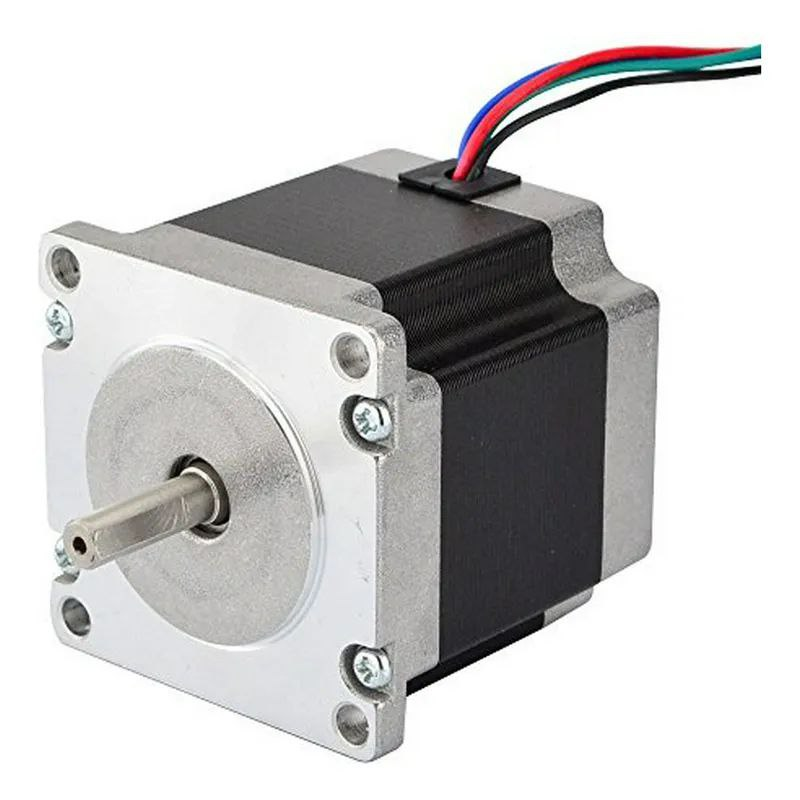
\includegraphics[height=4cm]{04-figuras/stepper-motor.jpg}
            \caption{Motor de paso}
            \label{fig:stepper-motor}
        \end{figure}

        El 23HS22-2804S es un motor paso a paso (stepper motor) híbrido, bipolar, diseñado para operar en sistemas de dos fases.

        Las características a tener en cuenta para su implementación en conjunto con el DM542T son:

        \begin{itemize}
            \item Corriente pico máxima de 2.8A (tabla \ref{tab:motor-especificaciones}).
            \item Torque máximo de 1.2Nm (tabla \ref{tab:motor-especificaciones}), según la carga a mover.
            \item Conexiones de las dos fases del motor descritas en la tabla \ref{tab:motor-tipo-conexiones}.
        \end{itemize}

    \subsection{Digital Stepper Drive DM542T.}

        \begin{figure}[H]
            \centering
            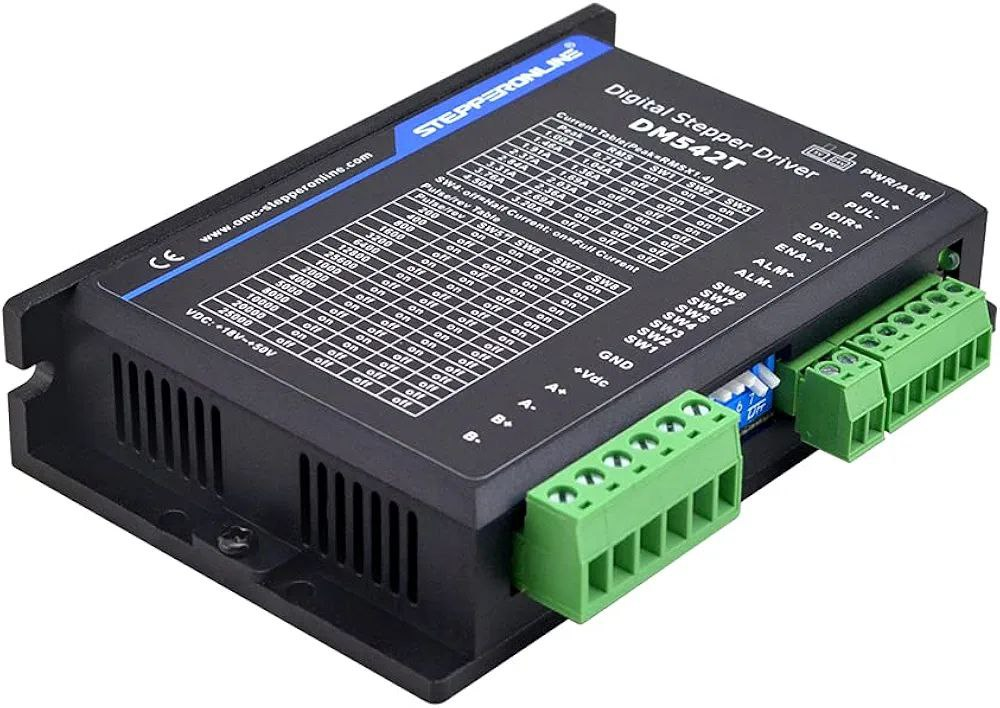
\includegraphics[height=4cm]{04-figuras/driver-motor.jpg}
            \caption{Controlador digital de motor de paso}
            \label{fig:driver-motor}
        \end{figure}

        El DM542T incluye las siguientes características clave según manual \cite{steeperonline}:

        \begin{itemize}
            \item Control de paso y dirección (PUL/DIR).
            \item Voltaje de entrada de 20-50VDC, con un rango recomendado de 24-48VDC.
            \item Frecuencia máxima de entrada de pulsos de 200 KHz.
            \item 16 resoluciones de micropasos de 200-25,600 configurables a través de interruptores DIP.
            \item 8 configuraciones de corriente de salida de 1.0-4.5A a través de interruptores DIP.
            \item Reducción de corriente en reposo (Idle current) seleccionable al 50\% o 90\% mediante el interruptor SW4.
            \item Auto-sintonización (*Auto-tuning*) para adaptarse a una amplia gama de motores paso a paso NEMA 11, 17, 23 y 24.
            \item Anti-Resonancia para un par óptimo, movimiento extra suave, y bajo calentamiento y ruido del motor.
            \item Arranque suave (*Soft-start*) sin "salto" al encenderse.
            \item Entradas ópticamente aisladas con opción de voltaje lógico de 5V o 24V.
            \item Salida de falla (*Fault output*).
            \item Protecciones integradas contra sobrevoltaje (activada cuando el voltaje de trabajo es mayor a 60VDC) y sobrecorriente.
        \end{itemize}

    \subsection{ROTATORY ENCODER (INCREMENTAL) E6B2-CWZ6C OMRON Corporation.}

        \begin{figure}[H]
        \centering
            \begin{subfigure}[b]{0.3\textwidth}
                \centering
                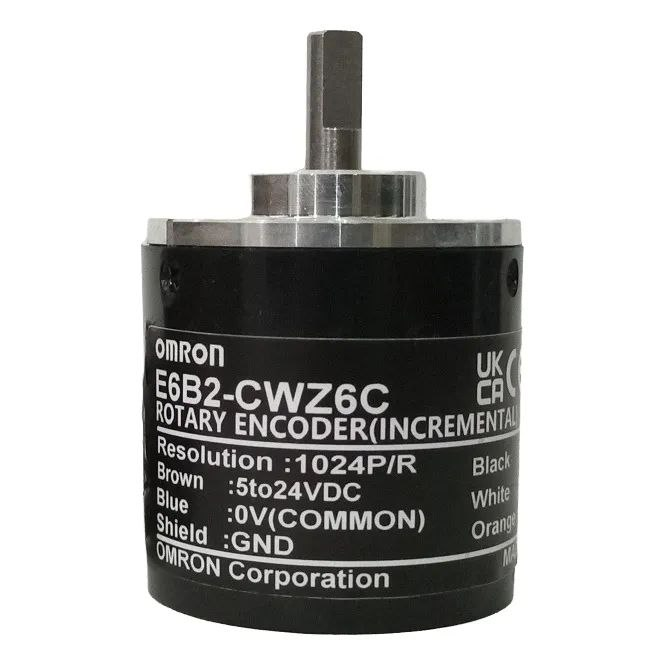
\includegraphics[width=\textwidth]{04-figuras/encoder.jpg}
                \caption{pines de alimentación.}
                \label{fig:encoderv1}
            \end{subfigure}
            \qquad
            \begin{subfigure}[b]{0.3\textwidth}
                \centering
                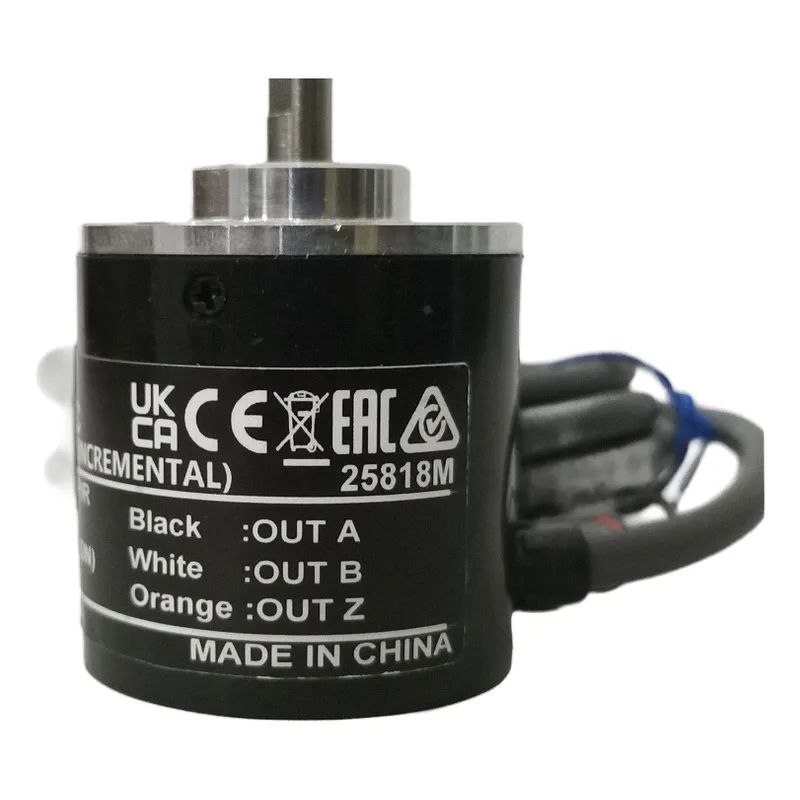
\includegraphics[width=\textwidth]{04-figuras/encoderv2.jpg}
                \caption{pines de fases.}
                \label{fig:encoderv2}
            \end{subfigure}
            \caption{Encoder rotativo} \label{fig:encoder}
        \end{figure}

        Se trata de un Codificador Rotatorio Incremental de propósito general, con la siguiente descripción, según hoja de datos \cite{omron}

        \begin{itemize}
            \item Ofrece un \textbf{amplio rango de voltaje de operación de 5 a 24 VCC} (para el modelo de colector abierto).
            \item Posee una \textbf{resolución de 1024 pulsos/revolución} en una carcasa de 40 mm.
            \item La \textbf{Fase Z se puede ajustar con facilidad} utilizando la función de indicación de origen.
            \item Está disponible un modelo con \textbf{salida de controlador de línea (line driver)} que permite que el cable se extienda hasta 100 m.
            \item Se permite una \textbf{carga mecánica grande} en la dirección radial de 29.4 N (3 kgf) y en la dirección de empuje de 19.6 N (2 kgf).
            \item El dispositivo opera con \textbf{fases de salida A, B y Z} (reversible).
            \item La \textbf{frecuencia máxima de respuesta} es de 100 kHz para el modelo E6B2-CWZ6C.
            \item Incorpora un \textbf{circuito de protección} contra cortocircuito de carga y conexión inversa para asegurar una operación altamente fiable (aplicable al modelo de colector abierto con salida de voltaje).
            \item La \textbf{velocidad máxima de revolución permitida} es de 6,000 rpm.
            \item La \textbf{temperatura ambiente de operación} va de –10°C a 70°C (sin formación de hielo).
            \item Posee un \textbf{grado de protección IEC60529 IP50}, aunque no es resistente al agua ni al aceite [8].
        \end{itemize}

        \begin{table}[H]
    \centering
    \caption{Características del encoder.}
    \begin{tabular}{|c|c|} \hline
        Especificación & Valor \\ \hline
        Resolución & 1024P/R \\
        Marrón & 5 a 24 VDC \\
        Azul & 0V (Común) \\
        Armadura & tierra (GND) \\
        Negro & Salida A \\
        Blanco & Salida B \\
        Naranja & Salida Z \\ \hline
    \end{tabular}
    \label{tab:encoder}
\end{table}

        \subsection{ESP32-WROOM-32}

        \begin{figure}[H]
            \centering
            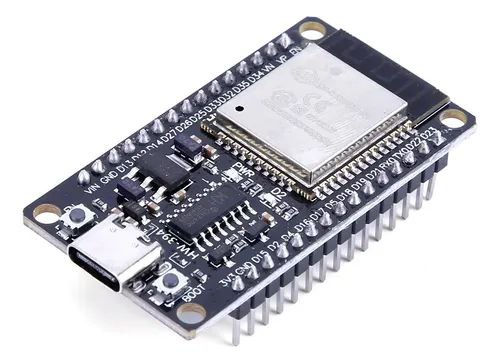
\includegraphics[height=4cm]{04-figuras/esp32.jpg}
            \caption{ESP32-WROOM-32}
            \label{fig:ESP32}
        \end{figure}

        El \textbf{ESP32-WROOM-32}, según \cite{esp32wroom32}, es un módulo MCU (Microcontroller Unit) genérico y potente que integra conectividad Wi-Fi, Bluetooth y Bluetooth LE. Está diseñado para ser utilizado en una amplia gama de aplicaciones, que abarcan desde redes de sensores que requieren bajo consumo de energía hasta tareas más exigentes, como la codificación de voz, la transmisión de música (*music streaming*) y la decodificación de MP3.

        En el núcleo del módulo se encuentra el chip \textbf{ESP32-D0WDQ6}, que utiliza un microprocesador Xtensa dual-core de 32 bits LX6, capaz de operar a una frecuencia de hasta 240 MHz. El módulo viene con una antena PCB integrada y 4 MB de flash SPI externo.

        \begin{itemize}
            \item \textbf{CPU y Memoria}
            \begin{itemize}
                \item Microprocesador Xtensa dual-core de 32 bits LX6, con hasta \textbf{240 MHz} de frecuencia.
                \item Incluye \textbf{448 KB de ROM}, \textbf{520 KB de SRAM} y \textbf{8 KB de SRAM} en el RTC (Reloj en Tiempo Real).
                \item Incorpora \textbf{4 MB de flash SPI}.
            \end{itemize}
            \item \textbf{Conectividad Inalámbrica}
            \begin{itemize}
                \item \textbf{Wi-Fi}: Soporta estándares 802.11b/g/n, con una tasa de bits de hasta 150 Mbps (802.11n).
                \item \textbf{Bluetooth}: Compatible con especificaciones \textbf{Bluetooth V4.2 BR/EDR} y \textbf{Bluetooth LE} (Bajo Consumo).
            \end{itemize}
            \item \textbf{Periféricos}
            \begin{itemize}
                \item Ofrece hasta \textbf{32 GPIOs} (incluyendo 5 GPIOs de *strapping*).
                \item Incluye interfaces \textbf{SD card, UART, SPI, SDIO, I2C}.
                \item Dispone de \textbf{controladores PWM} para LEDs y para Motores (Motor PWM).
                \item Incorpora \textbf{ADC} (Convertidor Analógico-Digital) y \textbf{DAC} (Convertidor Digital-Analógico).
                \item Cuenta con un \textbf{sensor táctil capacitivo}.
                \item Soporta la interfaz \textbf{TWAI\textregistered} (compatible con la Especificación CAN 2.0, según ISO 11898-1).
            \end{itemize}
            \item \textbf{Condiciones de Operación}
            \begin{itemize}
                \item Voltaje de operación/alimentación: \textbf{3.0 ~ 3.6 V}.
                \item Temperatura ambiente de operación: de \textbf{-40 a 85 °C}.
            \end{itemize}
        \end{itemize}

        Se incluye en los Anexos el pinout correspondiente al utilizado en el trabajo (fig. \ref{fig:esp32-pinout}) y el link correspondiente a la hoja de datos del mismo en la biblografía \cite{esp32wroom32}.

    \subsection{Pantalla LCD WH1602B 16 carácteres x 2 líneas.}

        \begin{figure}[H]
            \centering
            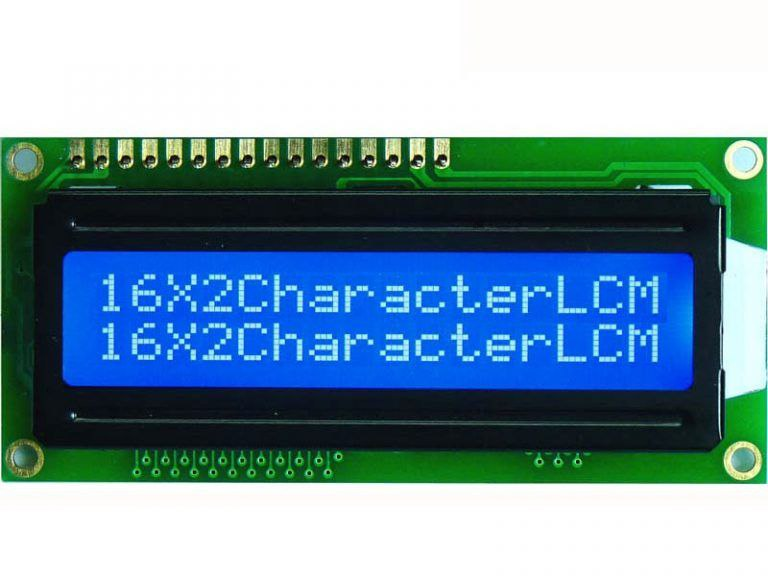
\includegraphics[height=4cm]{04-figuras/pantalla-lcd.jpg}
            \caption{Pantalla LCD.}
            \label{fig:pantalla-lcd}
        \end{figure}

        El módulo de visualización WH1602B \cite{WinstarLCD} es una pantalla LCD que presenta un formato de 16 caracteres por 2 líneas. Sus dimensiones son de 80.0 x 36.0 x 13.5 mm (máximo), con un área de visualización (View area) de 66.0 x 16.0 mm. Utiliza un backlight de tipo LED y está controlado por el circuito integrado IC ST7066U, comunicándose mediante una interfaz de la serie 68. En cuanto a sus requisitos eléctricos, opera con un voltaje de suministro lógico VDD-VSS de 4.5 a 5.5 V (típico 5.0 V), y está diseñada para funcionar en un amplio rango de temperatura operativa de -20 °C a +70 °C.

    \subsection{Adaptador I2C para pantalla LCD.}

        \begin{figure}[H]
            \centering
            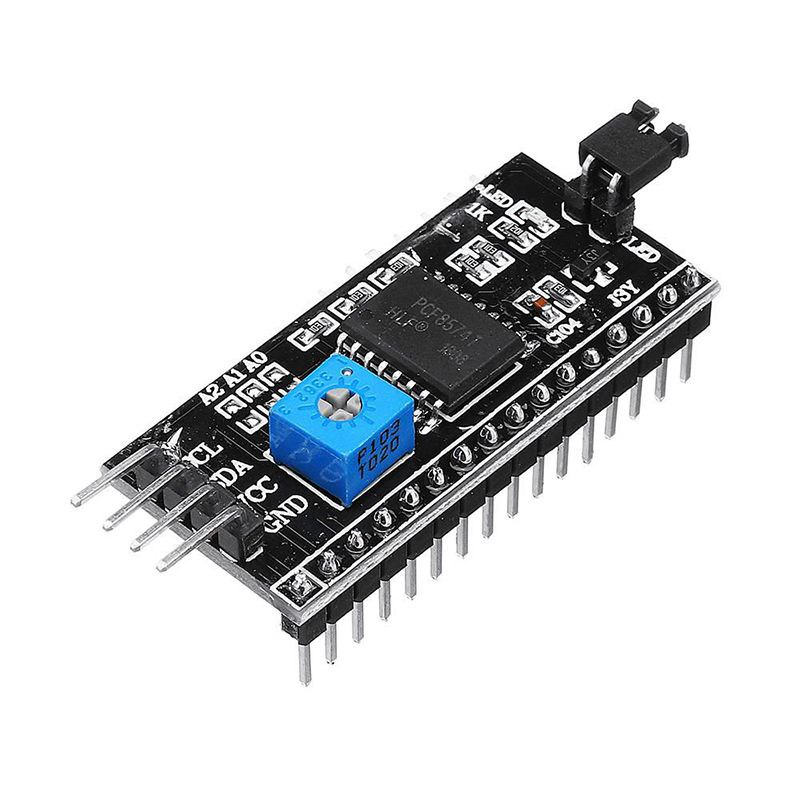
\includegraphics[height=4cm]{04-figuras/adaptador-i2c.jpg}
            \caption{Adaptador I2C.}
            \label{fig:adaptador-i2c}
        \end{figure}

        El modulo consiste en un diseño que utiliza el chip MCP23017 y es compatible con pantallas de cristal líquido de 1602 y 12864, a través de este módulo se cambia el bus habitual de comunicación a el uso I2C, para ello solo se necesitan dos I/Os del MCU para poder realizar el control de la pantalla de cristal líquido. El potenciómetro del módulo permite realizar un ajuste de contraste. También posee un jumper que controla el encendido de la retroiluminación o ajustar el brillo a través de PWM.

    \subsection{Convertidor DC DC Arduino basado en LM2596.}

        \begin{figure}[H]
            \centering
            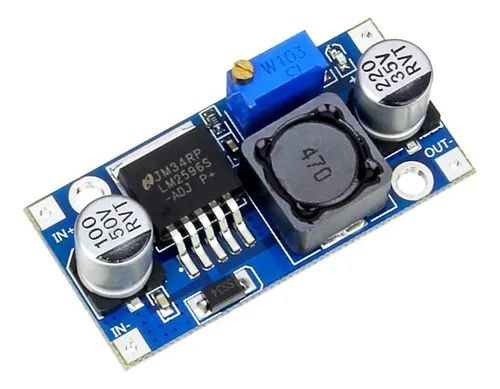
\includegraphics[height=4cm]{04-figuras/convertidor-dc-dc.jpg}
            \caption{convertidor LM2596.}
            \label{fig:convertidor-dcdc}
        \end{figure}

        El convertidor de voltaje DC-DC Step-Down 3A LM2596 tiene como función entregar un voltaje de salida constante inferior al voltaje de entrada frente a variaciones del voltaje de entrada o de carga. Soporta corrientes de salida de hasta 3A, voltaje de entrada entre 4.5V a 40V y voltaje de salida entre 1.23V a 37V. El voltaje de salida se selecciona mediante un potenciómetro multivuelta.
    
\section{Implementación de Encoder}



\section{Diagrama de Conexiones.}

\begin{figure}[H]
    \centering
    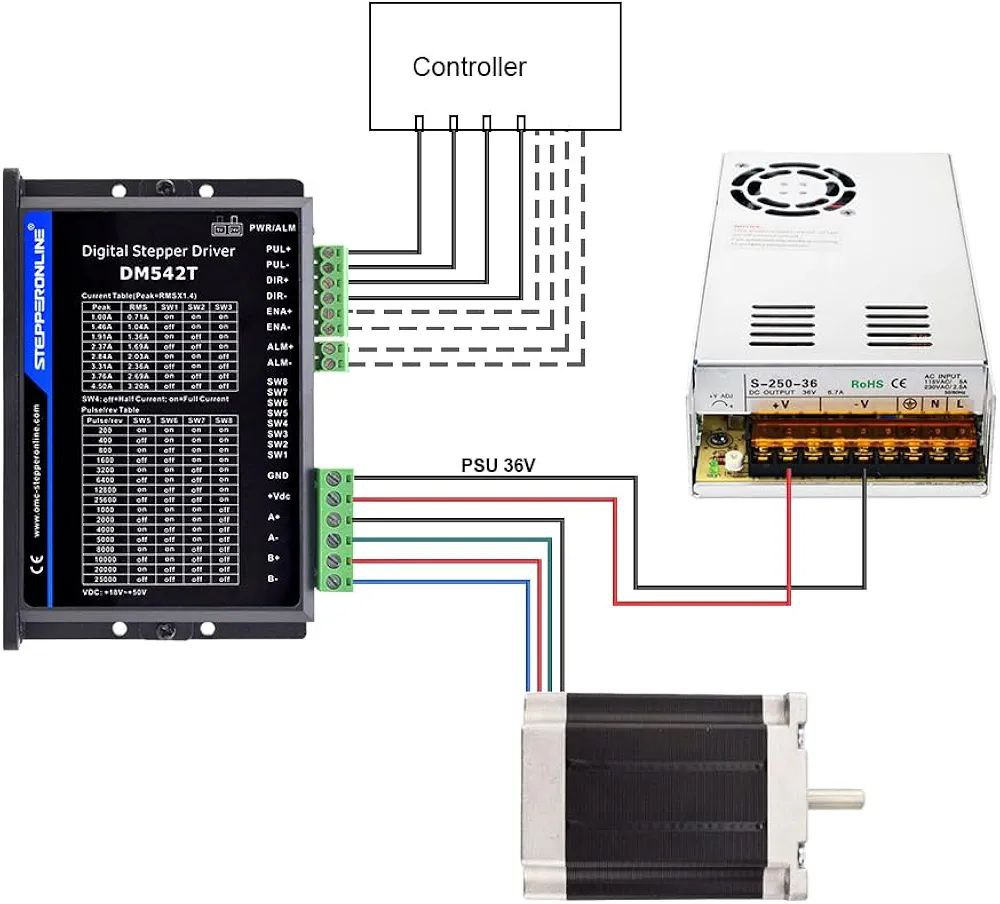
\includegraphics[width=\textwidth]{04-figuras/diagrama-motor.jpg}
    \caption{Diagrama de conexiones para utilizar motor.}
    \label{fig:diagrama-motor}
\end{figure}

\begin{figure}[H]
    \centering
    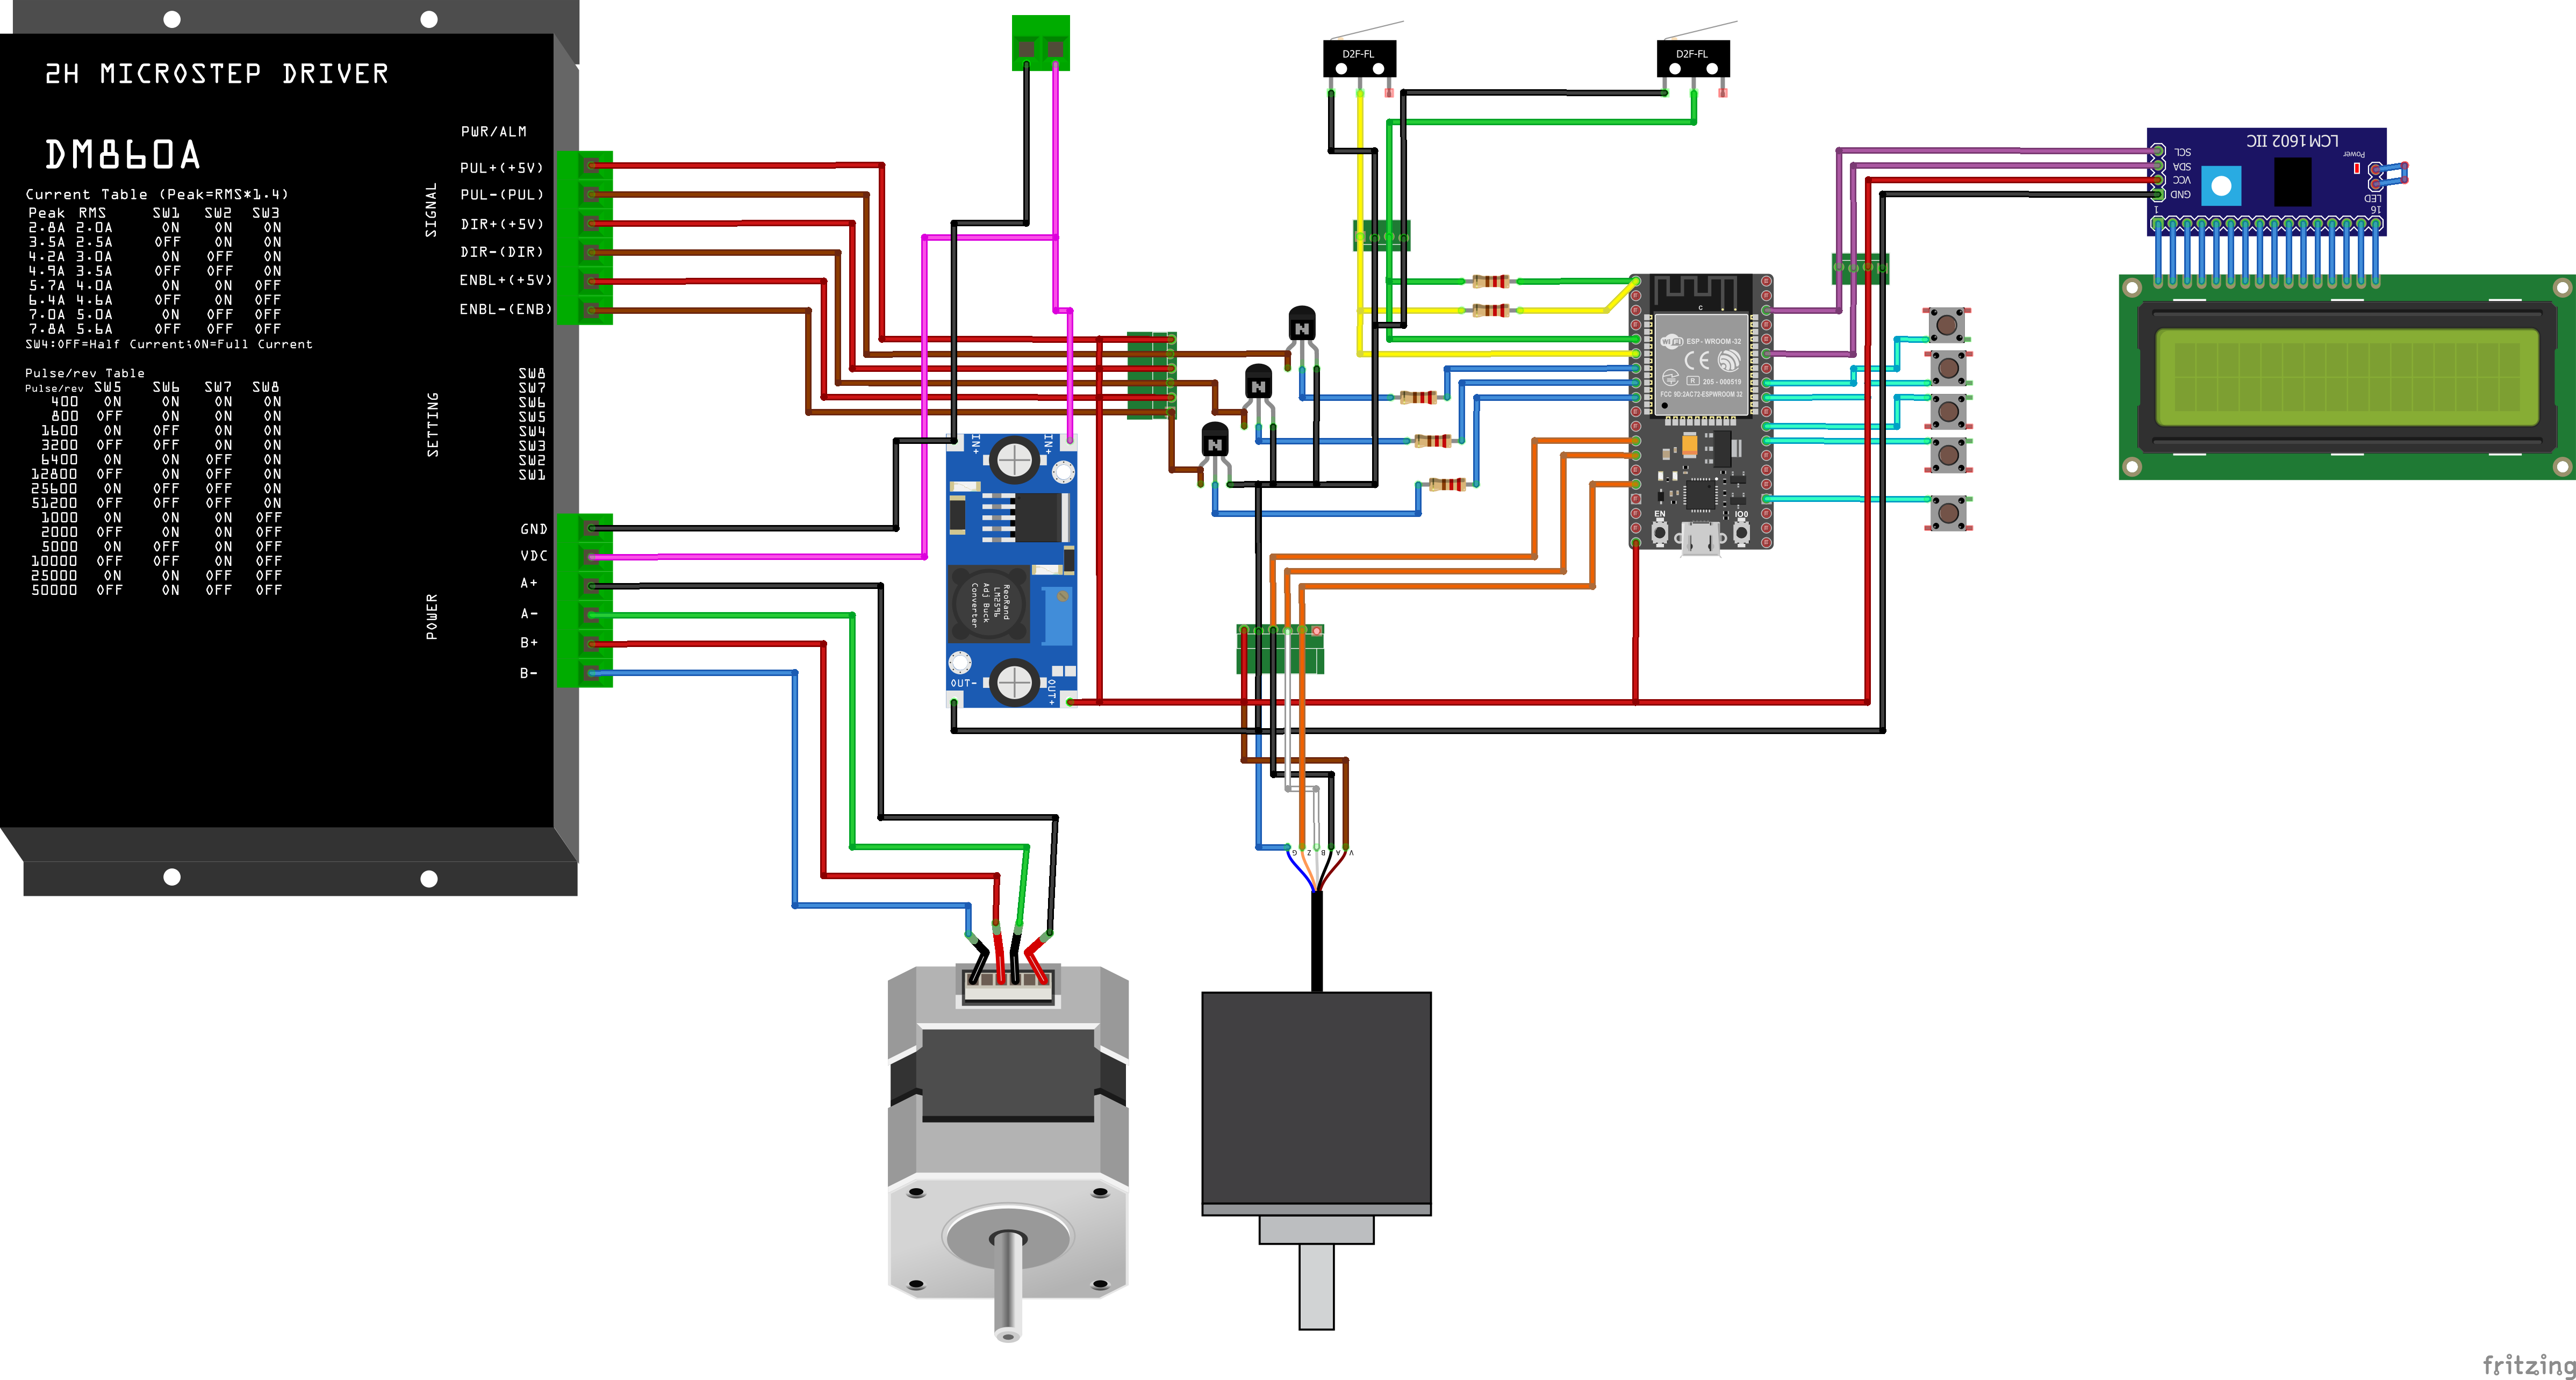
\includegraphics[width=\textwidth]{04-figuras/diagrama_conexion_control_bb.png}
    \caption{Diagrama de conexiones de sistema.}
    \label{fig:diagrama-completo}
\end{figure}